\section{ACSC Inverse Cosecant Function}

\subsection{Usage}

Computes the inverse cosecant of its argument.  The general
syntax for its use is
\begin{verbatim}
  y = acsc(x)
\end{verbatim}
where \verb|x| is an \verb|n|-dimensional array of numerical type.
\subsection{Function Internals}

The \verb|acosh| function is computed from the formula
\[
   \csc^{-1}(x) = \sin^{-1}\left(\frac{1}{x}\right)
\]
\subsection{Examples}

Here is a simple plot of the inverse cosecant function
\begin{verbatim}
--> x1 = -10:.01:-1.01;
--> x2 = 1.01:.01:10;
--> plot(x1,acsc(x1),x2,acsc(x2)); grid('on');
\end{verbatim}


\centerline{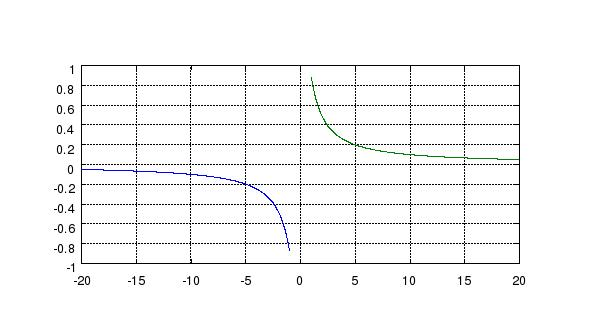
\includegraphics[width=8cm]{acschplot}}

